\documentclass[conference]{IEEEtran}
\IEEEoverridecommandlockouts
% The preceding line is only needed to identify funding in the first footnote. If that is unneeded, please comment it out.
%Template version as of 6/27/2024

\usepackage{cite}
\usepackage{float}
\usepackage{amsmath,amssymb,amsfonts}
\usepackage{algorithmic}
\usepackage{graphicx}
\usepackage{textcomp}
\usepackage{xcolor}
\usepackage{booktabs}
\usepackage{tabularx}
\usepackage{subcaption}


\def\BibTeX{{\rm B\kern-.05em{\sc i\kern-.025em b}\kern-.08em
    T\kern-.1667em\lower.7ex\hbox{E}\kern-.125emX}}
\begin{document}

\title{Design and Evaluation of  Two Spherical Systems for 3D Mapping*\\

\thanks{Identify applicable funding agency here. If none, delete this.}
}

\author{\IEEEauthorblockN{Marawan Khalil, Fabian Arzberger, and Andreas Nüchter}
\IEEEauthorblockA{\textit{Computer Science XVII – Robotics} \\
\textit{Julius-Maximilians-University}\\
Würzburg, Germany \\
marawan.khalil@stud-mail.uni-wuerzburg.de, \{fabian.arzberger, andreas.nuechter\}@uni-wuerzburg.de}
}

\maketitle

\begin{abstract}
This document is a model and instructions for \LaTeX.
This and the IEEEtran.cls file define the components of your paper [title, text, heads, etc.]. *CRITICAL: Do Not Use Symbols, Special Characters, Footnotes, 
or Math in Paper Title or Abstract.
\end{abstract}

\begin{IEEEkeywords}
component, formatting, style, styling, insert.
\end{IEEEkeywords}

\section{Introduction}
In recent decades, robotics has evolved from a niche discipline into a transformative technology impacting a wide range of industries, including manufacturing, healthcare, space exploration, and personal assistance. Among the diverse types of robotic systems, spherical robots have recently begun to attract increased attention from researchers. These robots represent a relatively unconventional design compared to more familiar, rotation-restricted systems such as UAVs, handheld devices, and wheeled vehicles. \\
\hspace*{1em}Unlike traditional wheeled or legged robots, spherical robots offer several key advantages, including omnidirectional movement, enhanced maneuverability in unpredictable environments, and improved protection for internal components. These features make them well-suited for a variety of applications such as surveillance, inspection, environmental monitoring in hazardous conditions, and search-and-rescue operations. Their spherical design enables them to access environments that are difficult or impossible for other robotic systems to navigate, such as steep tunnels, underground mines, narrow passageways, and other confined or dangerous spaces.
The sealed outer shell of a spherical robot provides full protection against dust, hazardous chemicals, liquids, and external impacts. Recent research has focused on developing more robust motion mechanisms \cite{roboball,novelsphere,pendulum_sphere} and incorporating technologies like LiDAR for 3D mapping, further expanding their capabilities in complex and unpredictable environments\cite{Kalman_filter_sphere,DAEDALUS,sphere_Fabi_1}.\\
\hspace*{1em}This research focuses on the development and evaluation of two custom-built spherical robots (see Fig. 1) equipped with advanced LiDAR-based SLAM systems. Both systems integrate Fast-LIO2\cite{fastlio2}, Fast-LIVO2\cite{fastlivo2}, and DLIO\cite{dlio}—state-of-the-art LiDAR-inertial odometry algorithms known for their real-time performance and accuracy.
In the next section, we review recent advancements in spherical robot design and the latest developments in SLAM for spherical platforms, with a particular emphasis on LiDAR-inertial methods. This is followed by a detailed description of the hardware implementation of the two spherical robots developed in this research. Subsequently, we describe the software integration, outlining the implementation of Fast-LIO2, Fast-LIVO2, and DLIO, as well as the motion control mechanisms used for the actuated sphere. Finally, we provide a comprehensive evaluation, comparing the proposed systems with existing solutions in terms of physical performance and mapping quality.

\begin{figure}[htbp]
\centerline{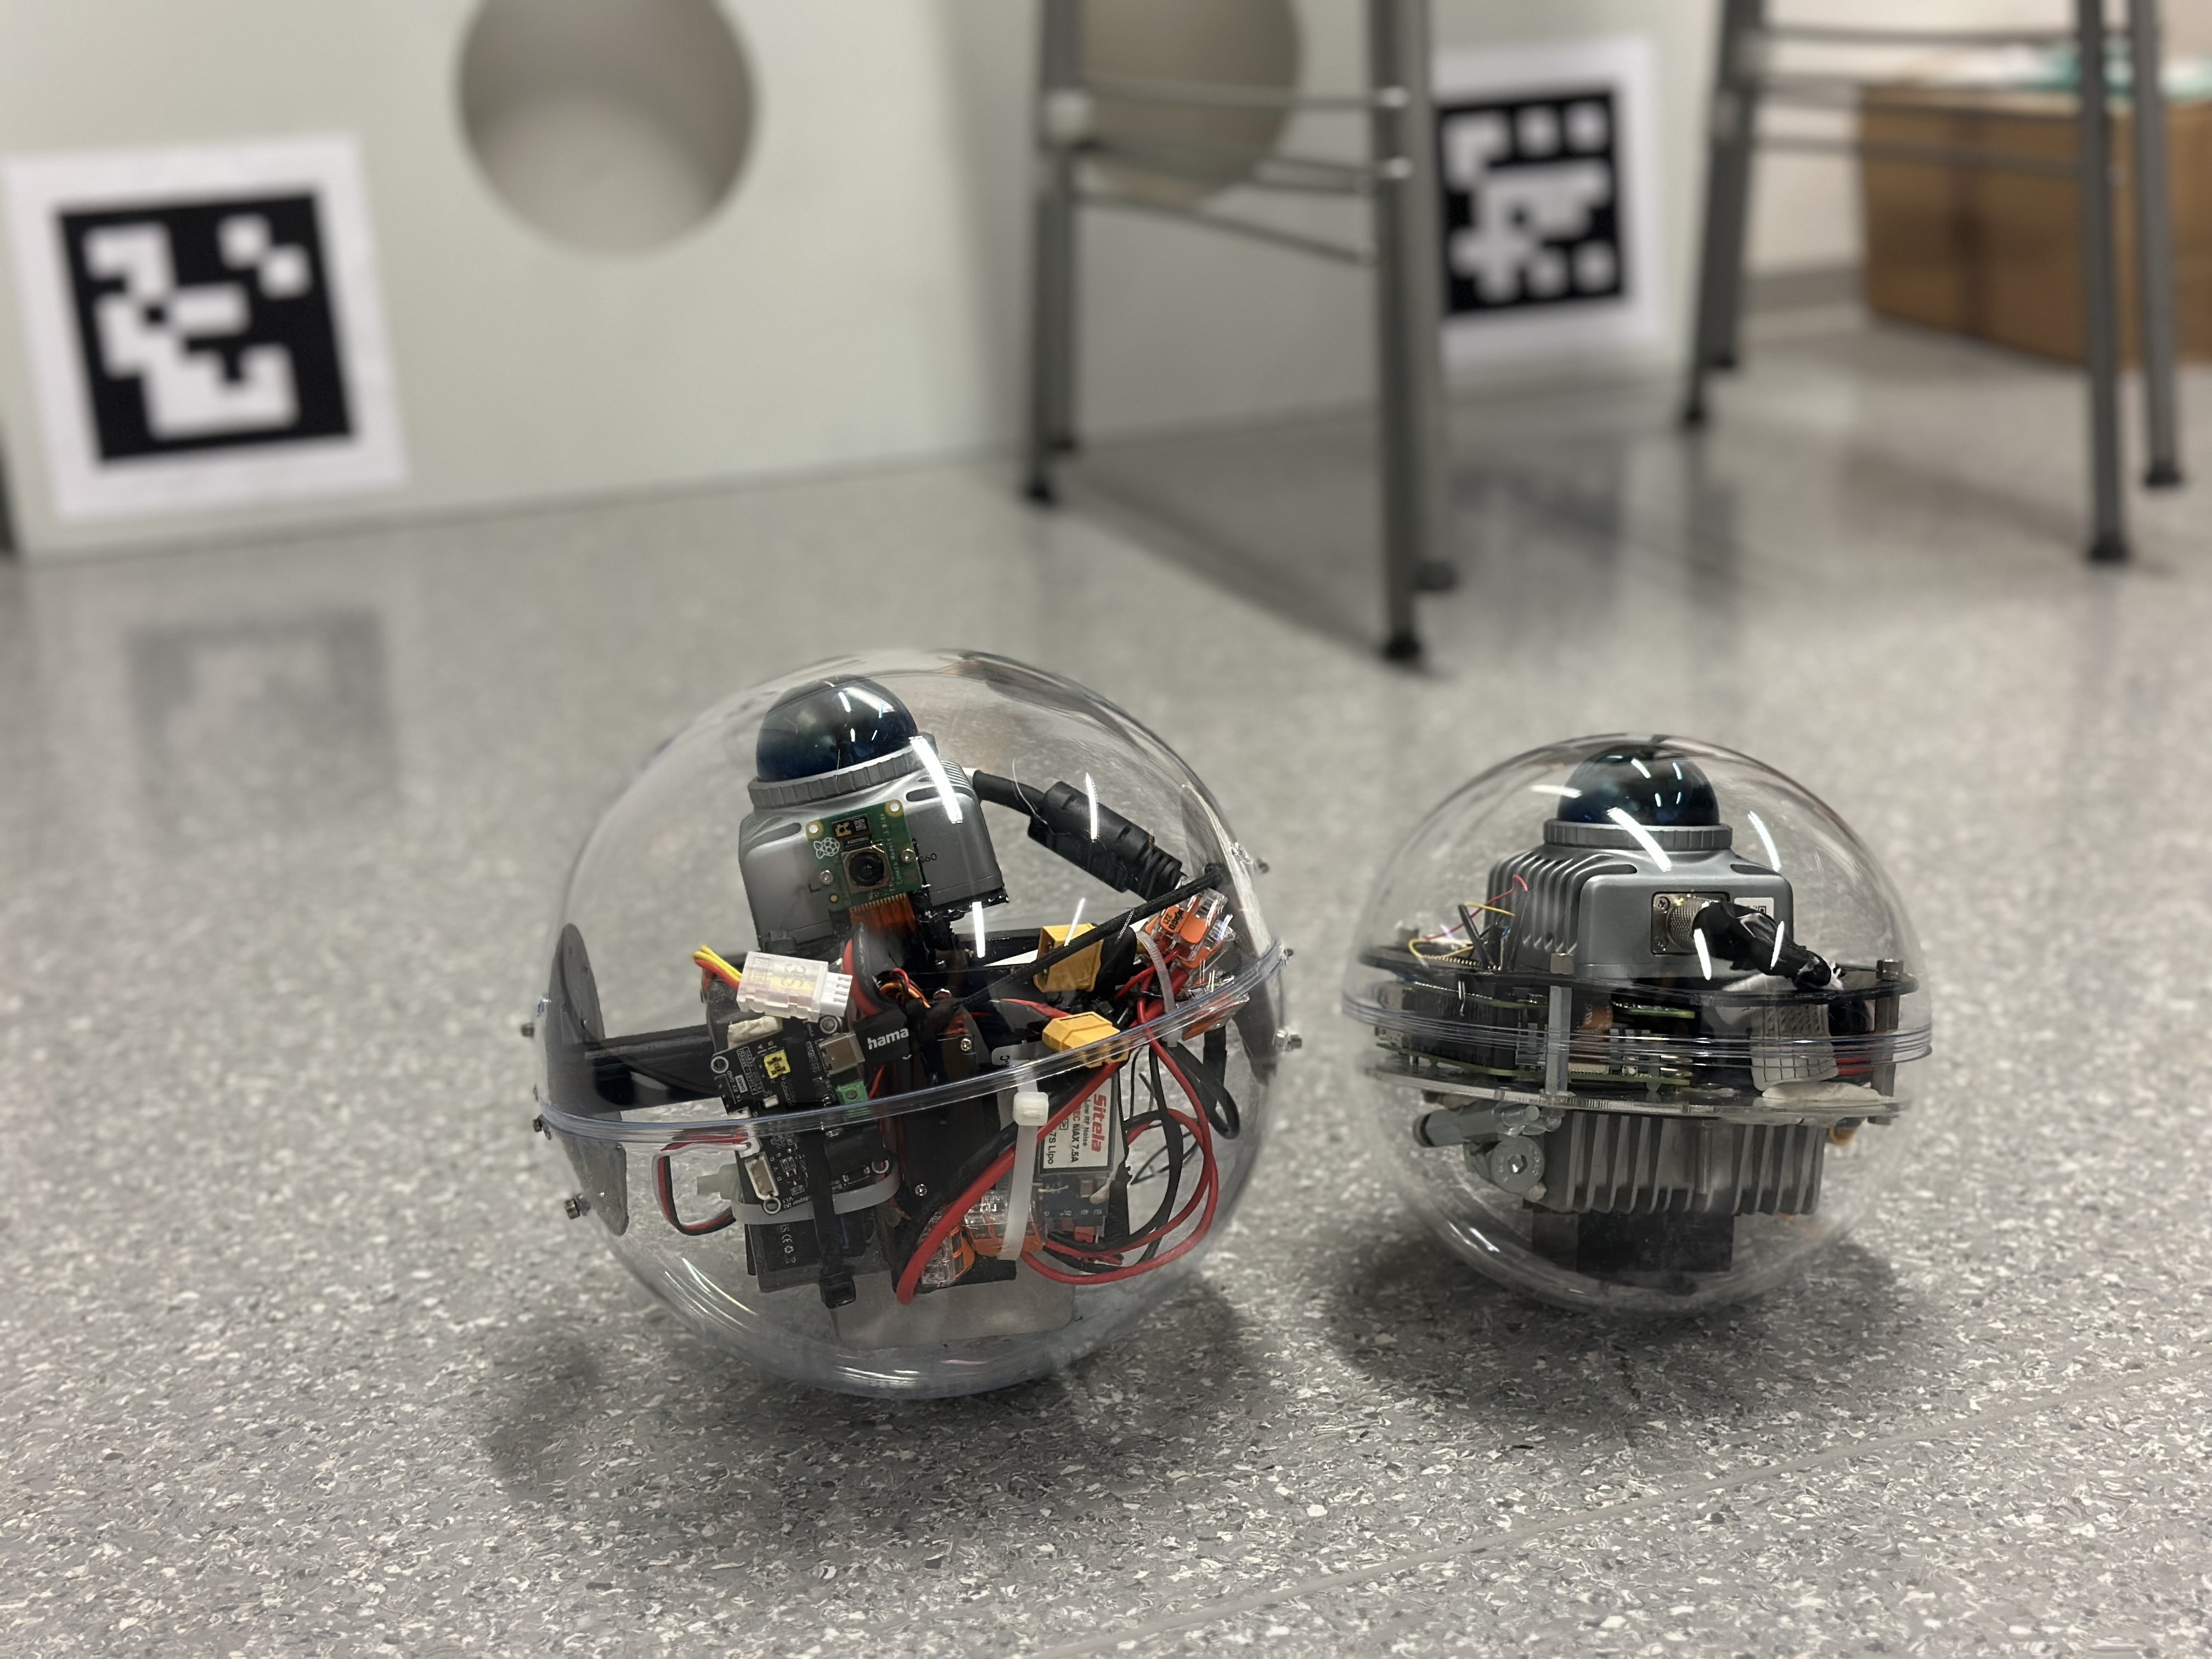
\includegraphics[width=0.9\columnwidth]{pics/two_spheres.jpg}}
\caption{(Left:) 20cm$\varnothing$ Actuated Sphere. (Right:) 16cm$\varnothing$ Non-actuated Sphere.}
\label{fig}
\end{figure}
\section{State of the Art}


\subsection{Spherical SLAM}\label{AA}

Spherical Simultaneous Localization and Mapping (SLAM) is an emerging area within mobile robotics, offering promising solutions for robust mapping in constrained or hazardous environments. Unlike traditional platforms, spherical robots encapsulate their sensors within a protective shell and rely on rolling locomotion. This unique configuration introduces both opportunities and significant challenges for SLAM algorithms. One of the earliest spherical SLAM prototypes was L.U.N.A. \cite{luna} , which employed a 2D LiDAR and IMU inside a rolling spherical shell. The design validated the feasibility of spherical SLAM. It also featured actuation through internal flywheels, using an IBCOAM (Impulse by Conservation of Angular Momentum) mechanism.
A major milestone in this field was the DAEDALUS project \cite{DAEDALUS}, funded by the European Space Agency, which proposed a fully enclosed spherical robot for the autonomous exploration of lunar lava tubes. The robot is suggested to be equipped with LiDAR and internal actuators, and its design focused on resilience to lunar regolith and harsh environmental conditions.\\
\hspace*{1em}A core challenge in spherical SLAM is the aggressive and non-centered rotation induced by rolling locomotion. These motions produce high angular velocities and dynamic behavior across all principal axes. This significantly degrades pose estimation accuracy and leads to error accumulation in the map. This problem is further compounded by the absence of magnetometer usage—often intentionally excluded due to the unreliability of magnetic field data in planetary environments—which leads to uncorrected yaw drift in IMU-based odometry, especially during prolonged navigation.\\
\hspace*{1em}To address these issues, Arzberger et al. \cite{Kalman_filter_sphere,sphere_Fabi_1,DeltaFilter} introduced specialized filtering techniques for spherical systems. Their Delta Filter is a lightweight, real-time, multi-trajectory pose estimation method that fuses unreliable trajectories—such as those from IMUs and stereo visual-inertial odometry (VIO)—into a more robust estimate, without requiring explicit sensor uncertainty modeling. The filter operates on pose changes ("deltas"), uses a probabilistic weighting scheme for translation estimation, and applies rotational interpolation via spherical linear interpolation (Slerp). A follow-up Kalman Filter design extended this approach by incorporating covariance-aware models, enhancing pose estimation accuracy during rapid and complex motion.\\
\hspace*{1em}Despite these advances, most current spherical SLAM systems still lack precise onboard actuation for controlled repositioning beyond rolling, limiting their effectiveness in tightly constrained environments. While recent studies (e.g. \cite{Kalman_filter_sphere}) have compared their results with state-of-the-art SLAM systems such as DLIO\cite{dlio} and FAST-LIO2\cite{fastlio2}, the field continues to evolve rapidly. Newer SLAM algorithms (e.g., FAST-LIVO2\cite{fastlivo2}), advanced LiDARs like the MID-360 and RoboSense Airy, and modern microprocessors such as the Raspberry Pi 5—with PCIe support and Gigabit Ethernet—are pushing the boundaries of what is possible. In this context, we introduce our first prototype, the Non-actuated Sphere, which leverages the processing power of the Raspberry Pi 5 16GB RAM model. This design enables offline SLAM on a compact spherical platform, while also extending battery life through improved power efficiency and reducing overall system cost.
\subsection{Spherical locomotion}

\label{sec:state-of-the-art}

Spherical locomotion has attracted significant research interest in recent years, driven by the pursuit of optimal mobility mechanisms. Although spherical robots may appear mechanically simple, a wide variety of locomotion strategies have been developed—and continue to emerge. One of the most well-known approaches is the Internal Driving Unit (IDU), or differential drive, used in commercial robots like the Sphero Bolt+ and BB-8. Akella et al.\cite{Sphero} analyzed BB-8’s internal wheel-driven system and demonstrated that effective control could be achieved using only two actuators. However, they highlighted a key limitation: the robot’s geometry inherently restricts it to rolling motion, preventing controlled sliding and reducing effectiveness on inclined or uneven terrain.\\

In contrast, Zevering et al.\cite{luna} introduced L.U.N.A., a spherical robot designed for autonomous 3D mapping in lunar caves. Rather than using wheels or rods, L.U.N.A. relies on internal flywheels to generate motion via the IBCOAM method. This approach enables a compact form factor and protects internal electronics—advantages particularly well suited to harsh and remote terrain. The robot demonstrated reliable motion on soft surfaces such as sand and rubber. However, limitations remain, including vibrational instability caused by unbalanced flywheels, reduced performance on inclined low-friction surfaces, and pose estimation errors due to unsynchronized sensor data.\\

In a following study by Zevering et al.\cite{rod_sphere} proposed a rod-driven spherical robot, also targeting lunar cave exploration. This design uses external linear actuators to push against the environment to induce motion. While it improves adaptability to rugged terrain and sharp obstacles, it introduces new challenges, such as oscillatory behavior from fixed-speed actuators, limited effectiveness on slopes, and the need for higher-power actuation when traversing dusty or soft ground.\\

Beyond differential and flywheel-based designs, several researchers have explored pendulum-driven locomotion due to its mechanical simplicity, energy efficiency, and natural stability. Oevermann et al. \cite{roboball}, Ren et al. \cite{novelsphere}, and  Kolbari et al. \cite{pendulum_sphere} developed spherical robots that use an internal heavy pendulum as the primary driving mechanism. While their configurations differ in terms of shell design and target applications, they share a common reliance on pendulum-based locomotion and have demonstrated robust movement across a variety of terrains.\\

A notable example is RoboBall\cite{roboball}, which features a novel soft pressurized shell and a two-degree-of-freedom internal pendulum. This robot successfully navigates gravel, grass, steep inclines, and even floats and maneuvers on water. However, the deformable shell introduces complex dynamic behaviors. These were addressed using a Linear Quadratic Regulator (LQR) for steering and a model-based proportional controller for driving. In contrast, \cite{novelsphere} and \cite{pendulum_sphere} adopted PID-based stabilization strategies to enhance motion control and responsiveness. RoboBall’s experiments further revealed that internal pressure and shell deformation significantly affect dynamic behavior—especially due to the presence of a “dead zone” where balance control becomes unstable during motion.\\

Taken together, these pendulum-based locomotion strategies highlight the value of combining mechanical simplicity with robust control to enable adaptive movement in unpredictable environments. While a variety of innovative locomotion methods have been proposed for spherical robots—including flywheel-, rod-, and pendulum-driven systems—most have been explored in isolation from modern SLAM techniques or have not been tested with active actuation. Although these designs demonstrate promising mobility across complex terrains, few have been evaluated in conjunction with advanced LiDAR-inertial odometry under real-world motion dynamics. This paper addresses this gap by introducing our second prototype—a pendulum-driven spherical robot designed to achieve both robust locomotion and accurate, real-time mapping performance within the constraints of a compact platform.

\section{Hardware and Design}

\subsection{Non-Actuated Sphere}

The non-actuated sphere was modeled using CAD software, drawing inspiration from \cite{Kalman_filter_sphere} design. Its structure consists of two flat discs stacked vertically and secured with pillar screws, maintaining a gap of approximately 28\,mm between them. The diameter of the discs was calculated using the Pythagorean theorem\eqref{Pythagorean} to ensure proper spacing and balance:

\begin{equation}
    d = \sqrt{h^2 + r^2} \label{Pythagorean}
\end{equation}


\noindent
where $d$ is the disc diameter, $h$ is the vertical spacing between the discs, and $r$ is the horizontal offset required to enclose internal components symmetrically.

To enhance structural integrity and safety, fillets were applied to the edges of the discs. Each disc has a uniform thickness of 3\,mm.

Two fabrication methods were used to produce the discs: 3D printing with PLA and laser cutting with acrylic. Both materials demonstrated sufficient durability during initial testing.

The below list summarizes the components used in the non-actuated sphere and its location within the sphere:



\begin{table}[H]
\centering
\caption{Hardware Components and Their Placement Inside the Sphere}
\label{tab:hardware_components}
\begin{tabularx}{\linewidth}{@{}l X@{}}
\toprule
\textbf{Layer} & \textbf{Components} \\
\midrule
Top    & Livox Mid-360 LiDAR, BNO-085 IMU \\
Middle & Raspberry Pi 5 (16 GB, 256 GB SSD, cooling fan) \\
       & 2200 mAh 3S LiPo battery \\
Bottom & Voltage regulators \\
\bottomrule
\end{tabularx}
\end{table}

\begin{figure}[htbp]
\centering
\begin{subfigure}{0.45\columnwidth}
    \centering
    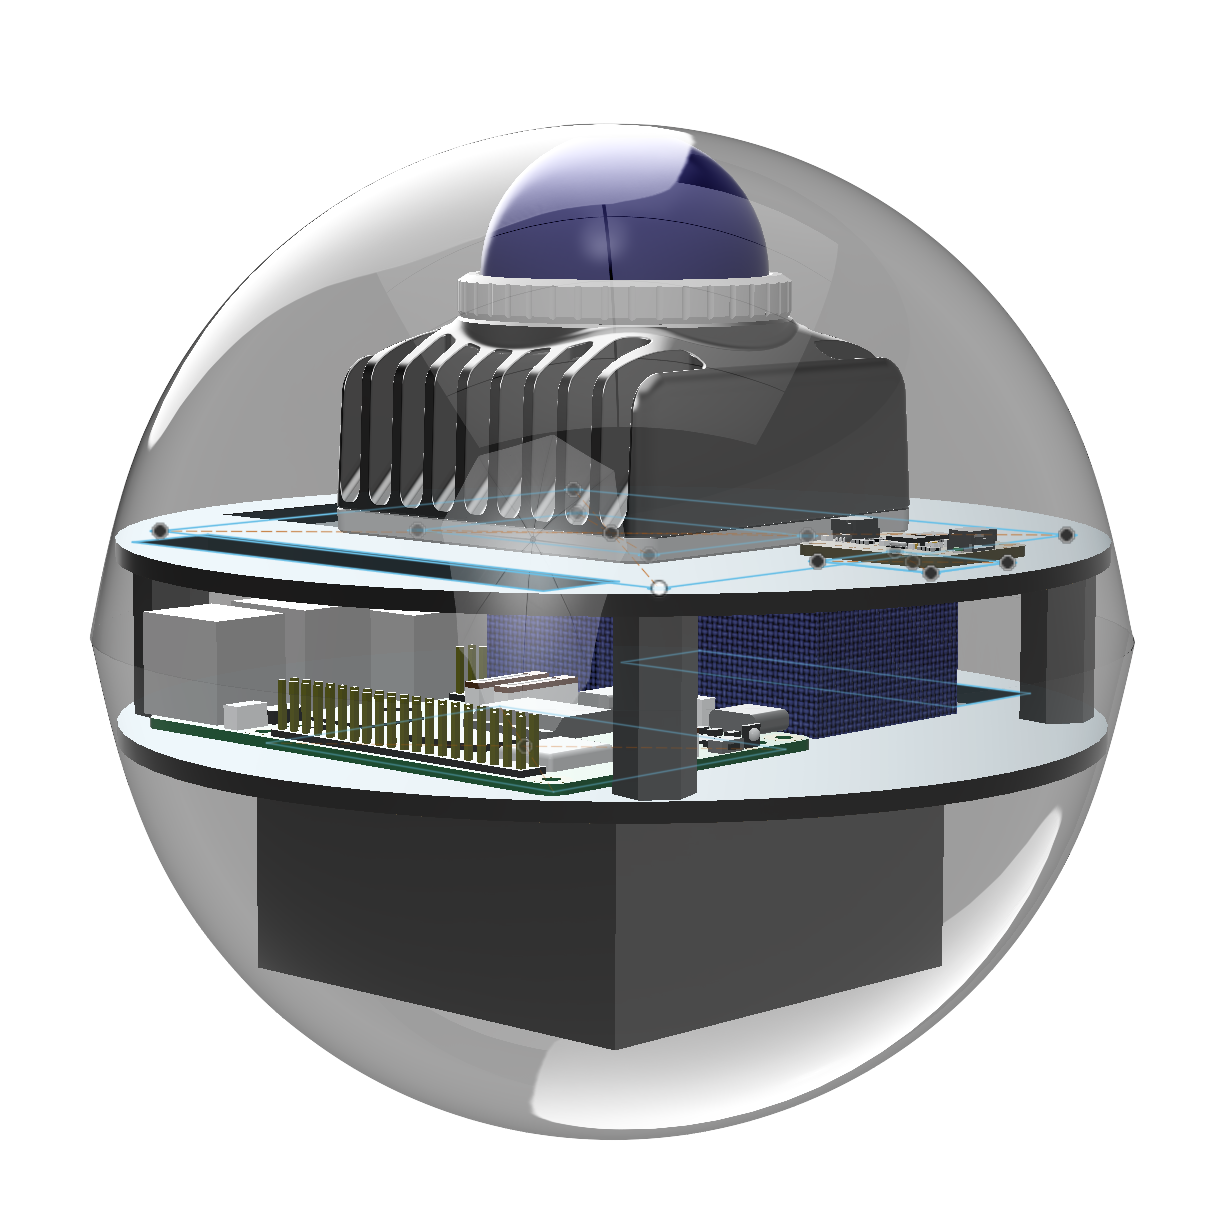
\includegraphics[width=\textwidth]{pics/Non_actuated_Sphere_CAD.png}
    \caption{3D CAD Model}
    \label{fig:cad-model}
\end{subfigure}
\hfill
\begin{subfigure}{0.45\columnwidth}
    \centering
    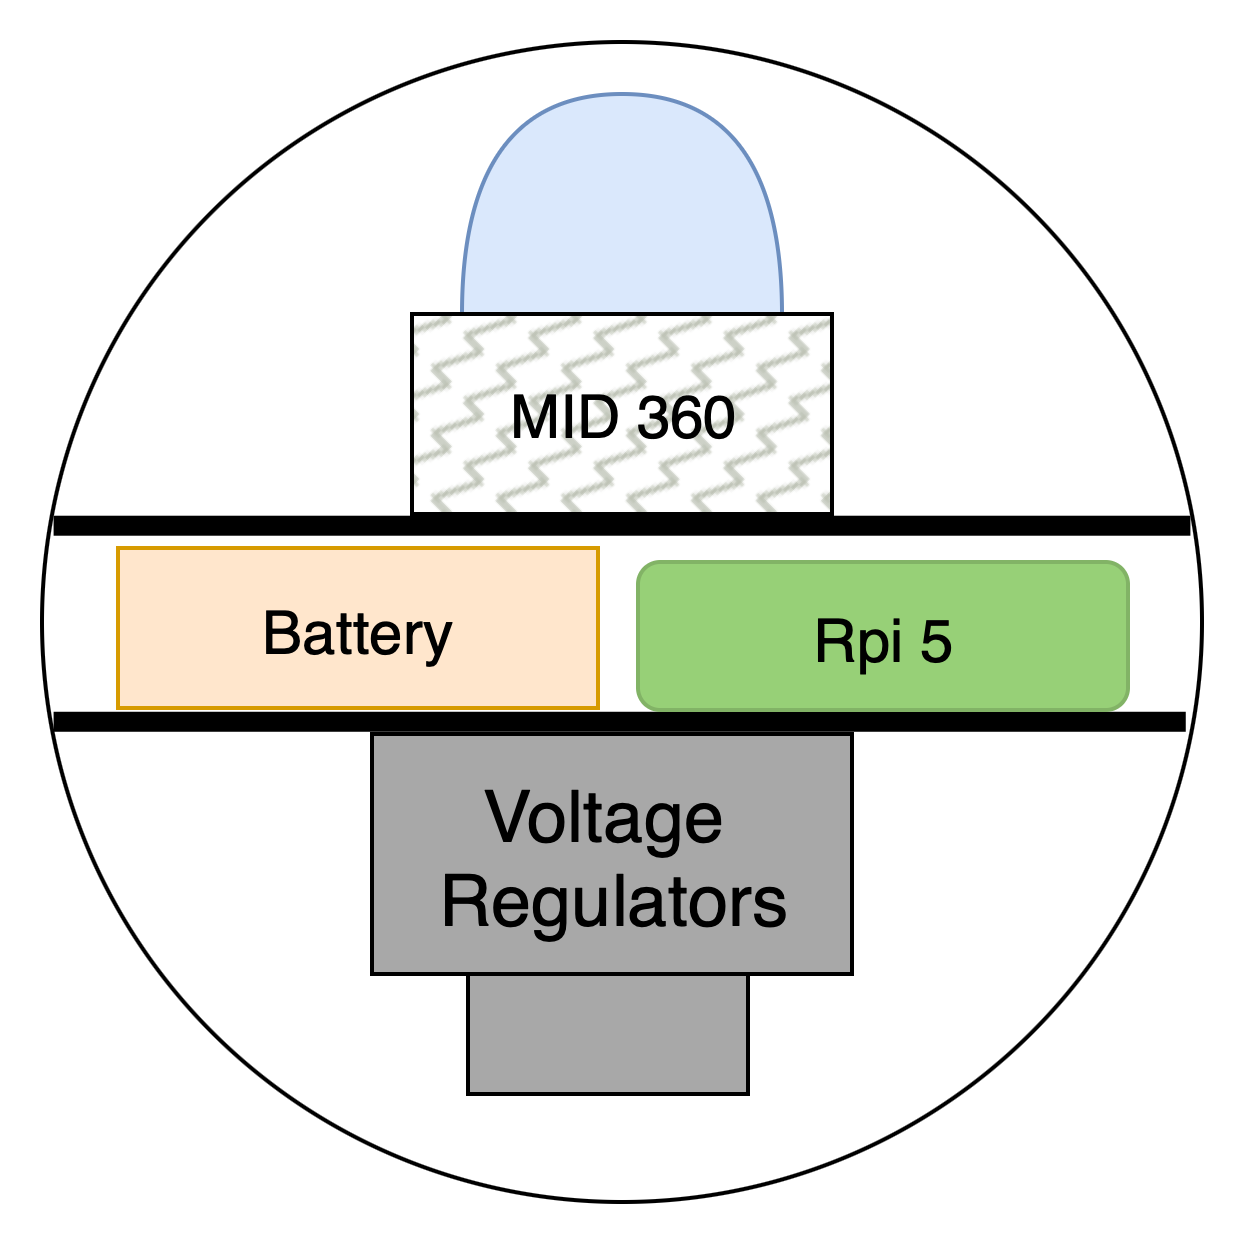
\includegraphics[width=\textwidth]{pics/image.png}
    \caption{Simplified 2D Model}
    \label{fig:2d-model}
\end{subfigure}
\caption{Different views of the Non-actuated sphere.}
\label{fig:cad-design1}
\end{figure}

The Livox Mid-360 is connected to the Raspberry Pi via Ethernet, while the BNO-085 IMU communicates using the I2C interface. 

The sphere is designed to be lightweight, with a total weight of approximately "X" kg, including the battery and all internal components. The sphere's diameter is 16 cm, making it compact and easy to transport. It is designed to be rolled manually by foot or hand.

To ensure stable and predictable rotation, metal weights were strategically placed within the sphere to align its center of mass with its geometric center. A 3D CAD model of the assembled structure is shown in fig.~\ref{fig:cad-design1}.



\subsection{Actuated Sphere}

The actuated sphere was designed using CAD software, with fig.~\ref{fig:cad-design2} illustrating the final structure. As described in Section~\ref{sec:state-of-the-art}, the design was inspired by the pendulum-driven locomotion mechanisms presented in studies~\cite{roboball, novelsphere}.

Unlike the non-actuated version, this sphere features an internal actuation system. At its core, a Waveshare Smart Continuous Servo (model ST3215) is mounted to control forward and backward motion by dynamically shifting the internal center of mass in the direction of travel. A second PWM-controlled servo enables left and right movement via pendulum displacement along the lateral axis.

The structural components were fabricated using PLA filament and 3D-printed in three separate pieces, which are then assembled into the complete sphere.


\begin{figure}[htbp]
\begin{subfigure}{0.45\columnwidth}
    \centering
    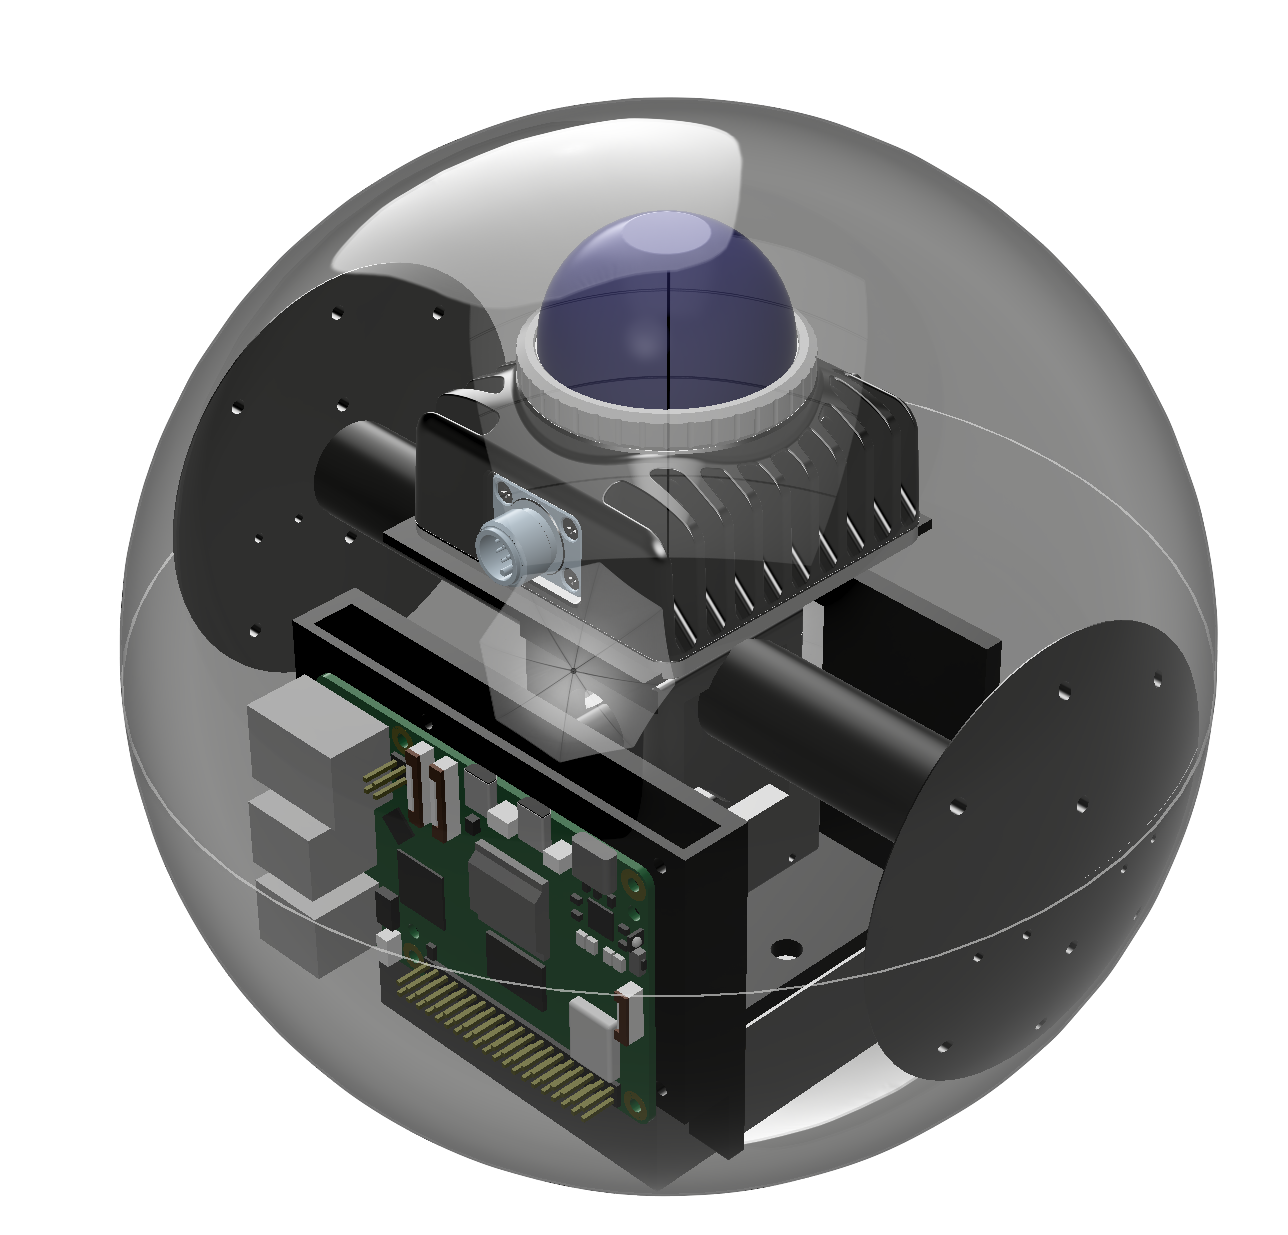
\includegraphics[width=\textwidth]{pics/Actuated_sphere.png}
    \caption{3D CAD model}
    \label{fig:cad-design2}
\end{subfigure}
\hfill
\begin{subfigure}{0.5\columnwidth}
    \centering
    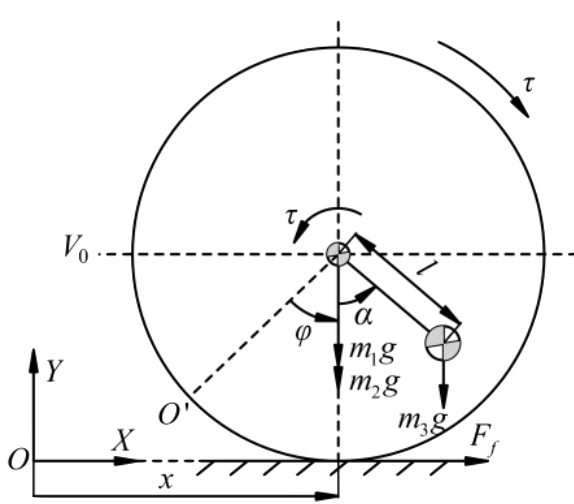
\includegraphics[width=\textwidth]{pics/planer_model.png}
    \caption{Simplified 2D Model}
    \label{fig:2d-model2}
\end{subfigure}
\caption{Different views of the Actuated sphere.}
\label{fig:cad-design2}
\end{figure}

The system dynamics involve key parameters including the robot’s horizontal position \( x \), the spinning angle of the shell \( \phi \), the swinging angle of the counter-weight mass \( \alpha \), and the input torque of the primary motor \( \tau \). Associated physical properties include the shell mass \( m_1 \), inner driver mass \( m_2 \), counter-weight mass \( m_3 \), gravitational acceleration \( g \), and the length of the connecting rod \( l \). All of this is taken into consideration when designing the sphere and its control system.
\\

\begin{figure*}[!t]
    \centering
    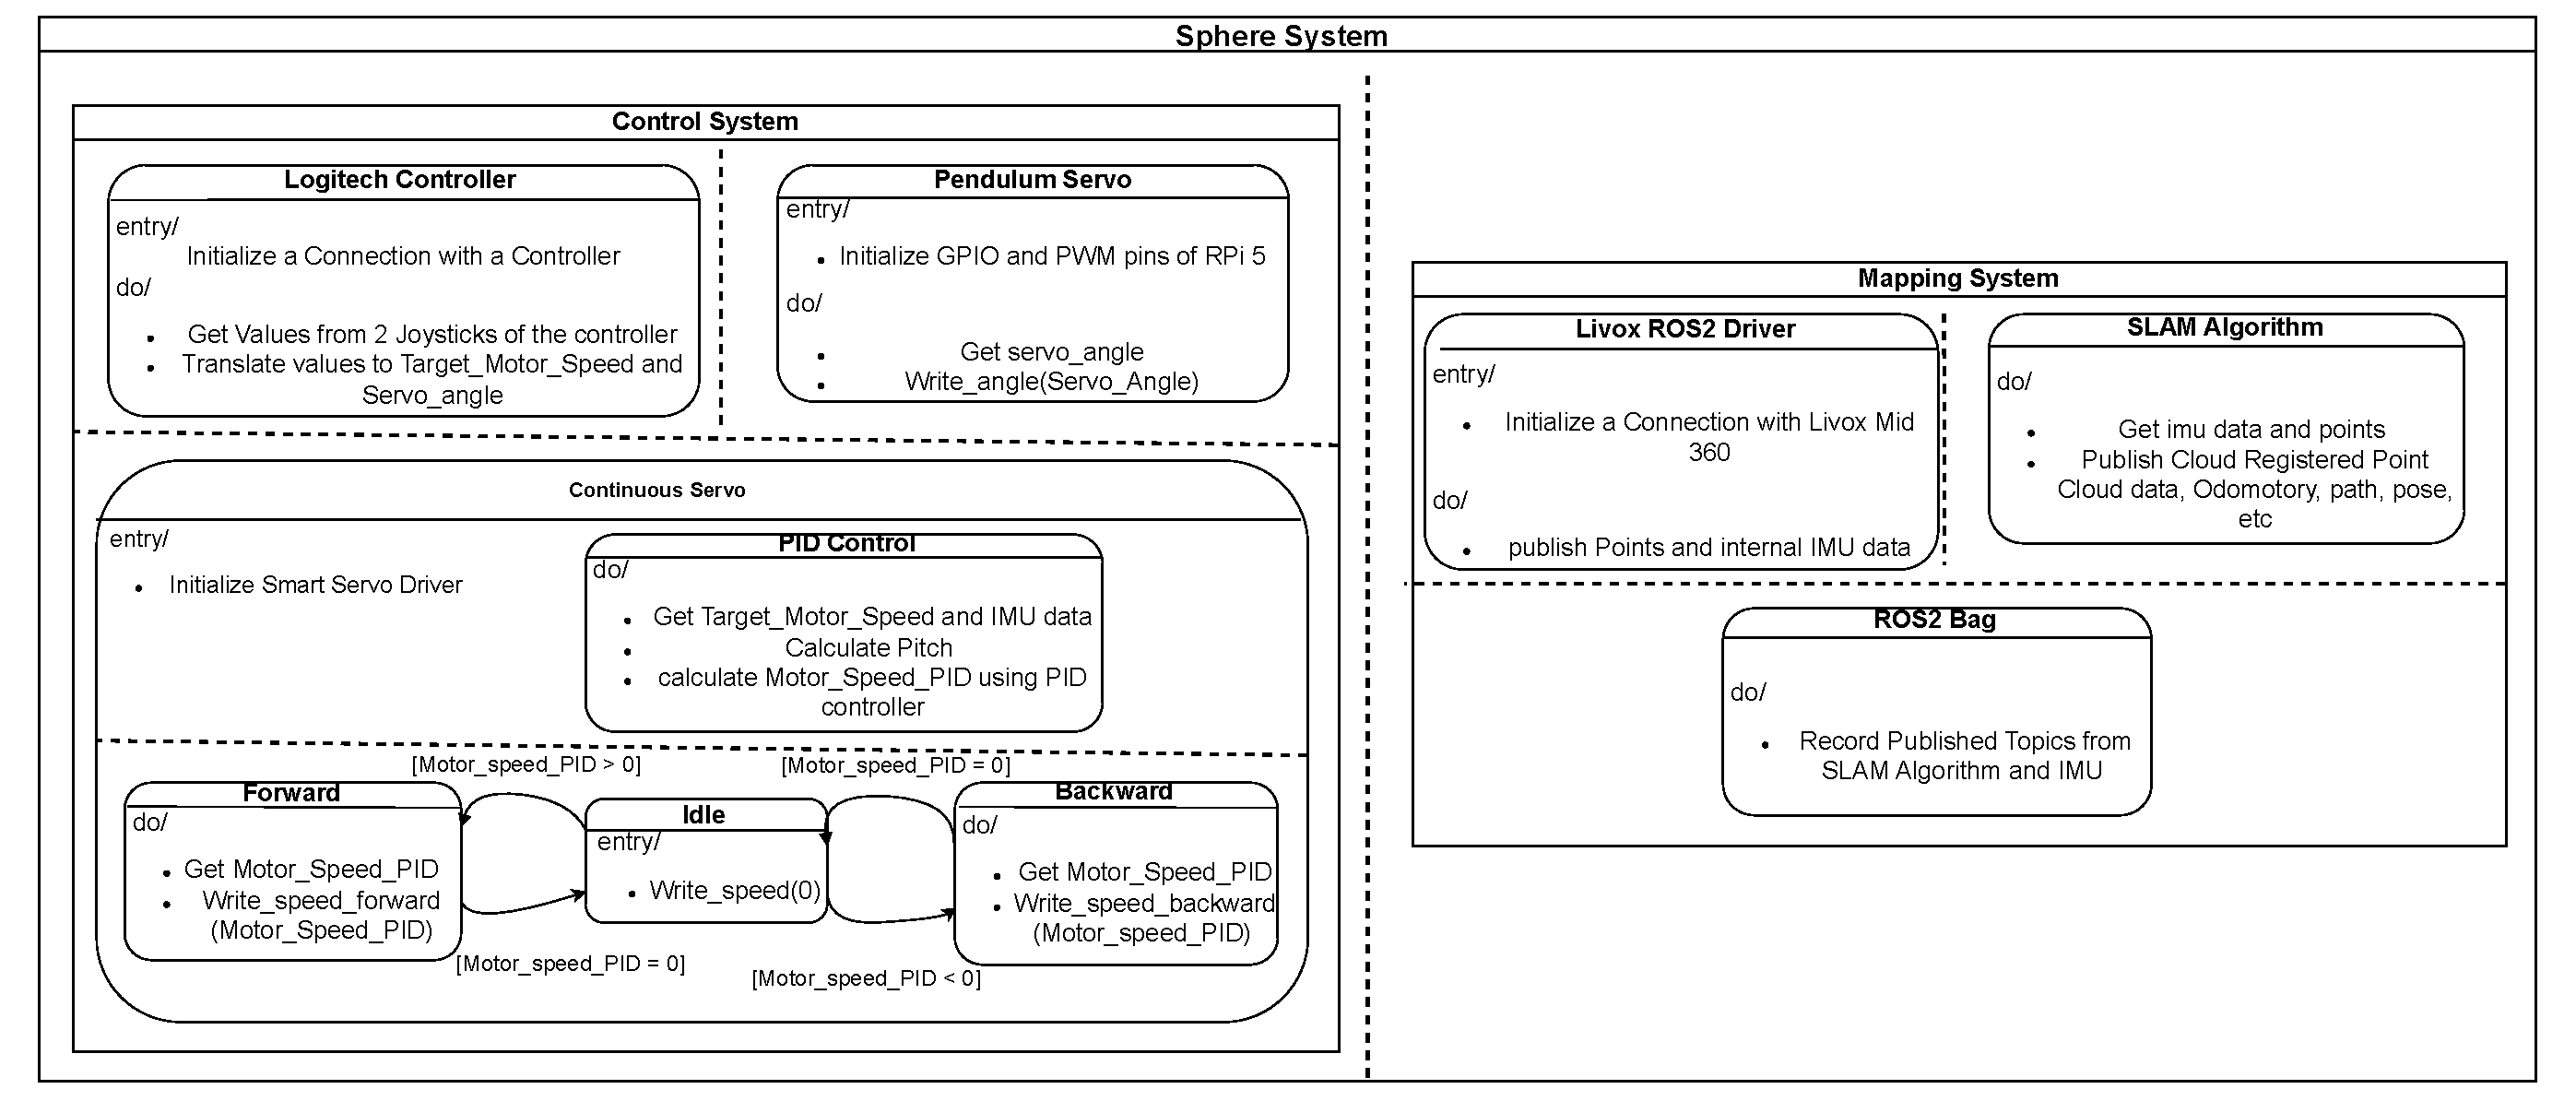
\includegraphics[width=1\linewidth]{pics/Khonsu.pdf} 
    \caption{State chart of the Sphere System showing the control and mapping subsystems.}
    \label{fig:sphere_system}
\end{figure*}

The internal hardware components are organized as follows:

\begin{table}[H]
\centering
\caption{Hardware Components and Their Placement Inside the Sphere}
\label{tab:hardware_components}
\begin{tabularx}{\linewidth}{@{}l X@{}}
\toprule
\textbf{Position} & \textbf{Components} \\
\midrule
Center & Waveshare Smart Continuous Servo (model ST3215) \\
       & Forward/backward actuation \\
       & PWM Servo – left/right pendulum control \\
Rear   & 2200 mAh 3S LiPo battery \\
       & 5V 5A voltage regulator (for Raspberry Pi 5) \\
       & 6V UBEC (for servo motors) \\
Pendulum Module & 12V 20A voltage regulator – powers the entire system; positioned near the shell for stability \\
Front  & Raspberry Pi 5 (16 GB model) \\
Top    & Livox Mid-360 LiDAR \\
       & Pi Camera V3 (12 MP) \\
\bottomrule
\end{tabularx}
\end{table}







\section{Software and Control System}


As shown in the system state diagram fig.~\ref{fig:sphere_system}, both the actuated and non-actuated spheres follow the same state transitions, with the exception of the control subsystem, which is unique to the actuated variant. All software components are deployed on Ubuntu 24.04.2 LTS ARM and ROS 2 Jazzy .

\subsection{Mapping System}

Both spheres incorporate a real-time mapping system. The following LiDAR-Inertial Odometry (LIO) frameworks were evaluated and integrated:

\begin{itemize}
    \item \textbf{FAST-LIO2}
    \item \textbf{DLIO}
    \item \textbf{FAST-LIVO2} (used in LIO-only mode)
\end{itemize}

Each system was configured and, where necessary, modified at the code level to meet the constraints and processing capabilities of the Raspberry Pi 5 and ROS2 Jazzy. All mapping computations are performed \textit{entirely onboard}, with no reliance on external computational resources. Resulting maps are stored in ros bag format for later evaluation and comparison against ground truth data.

\subsection{Actuator System (Actuated Sphere Only)}

The actuated sphere features an internal movement control system, operated using a  Logitech F710 controller. The controller's two joysticks are mapped to distinct control tasks:



\begin{itemize}
    \item \textbf{Servo control:} One joystick provides input to the continuous rotation servo. These inputs are scaled and passed through a discrete PID (Proportional-Integral-Derivative) controller to regulate pitch by minimizing the error between a desired target angle and the current angle measured by the IMU. The control signal is computed as

\[
u[k] = K_p \cdot e[k] + K_i \cdot \sum_{i=0}^{k} e[i] \cdot \Delta t + K_d \cdot \frac{e[k] - e[k-1]}{\Delta t}
\]

where \( u[k] \) is the servo motor command at time step \( k \), \( e[k] \) is the pitch error defined as the difference between the target angle \( \theta_{\text{target}} \) and the current angle \( \theta_{\text{current}} \), and \( K_p \), \( K_i \), \( K_d \) are the proportional, integral, and derivative gains, respectively. The controller runs at a fixed sampling interval \( \Delta t \) and includes a small deadband around the setpoint to reduce oscillations. Within this deadband, the integral term is reset to prevent windup. Additionally, manual control inputs can be superimposed onto the PID output, enabling user intervention without disrupting balance. The resulting command is then limited to a predefined range before being sent to the servo motor.
, which also considers real-time motor speed and IMU feedback to maintain stable velocity and orientation.
    \item \textbf{Mass shifting:} The second joystick adjusts the angle of an internal weight to shift the center of mass left or right, enabling directional control of the sphere's rolling behavior.
\end{itemize}

This control strategy allows for fine-grained movement and stabilization, combining feedback-based servo control with physical mass displacement for maneuvering.


\section{Evaluation and Results}

\subsection{\LaTeX-Specific Advice}

Please use ``soft'' (e.g., \verb|\eqref{Eq}|) cross references instead
of ``hard'' references (e.g., \verb|(1)|). That will make it possible
to combine sections, add equations, or change the order of figures or
citations without having to go through the file line by line.

Please don't use the \verb|{eqnarray}| equation environment. Use
\verb|{align}| or \verb|{IEEEeqnarray}| instead. The \verb|{eqnarray}|
environment leaves unsightly spaces around relation symbols.

Please note that the \verb|{subequations}| environment in {\LaTeX}
will increment the main equation counter even when there are no
equation numbers displayed. If you forget that, you might write an
article in which the equation numbers skip from (17) to (20), causing
the copy editors to wonder if you've discovered a new method of
counting.

{\BibTeX} does not work by magic. It doesn't get the bibliographic
data from thin air but from .bib files. If you use {\BibTeX} to produce a
bibliography you must send the .bib files. 

{\LaTeX} can't read your mind. If you assign the same label to a
subsubsection and a table, you might find that Table I has been cross
referenced as Table IV-B3. 

{\LaTeX} does not have precognitive abilities. If you put a
\verb|\label| command before the command that updates the counter it's
supposed to be using, the label will pick up the last counter to be
cross referenced instead. In particular, a \verb|\label| command
should not go before the caption of a figure or a table.

Do not use \verb|\nonumber| inside the \verb|{array}| environment. It
will not stop equation numbers inside \verb|{array}| (there won't be
any anyway) and it might stop a wanted equation number in the
surrounding equation.

\subsection{Some Common Mistakes}\label{SCM}
\begin{itemize}
\item The word ``data'' is plural, not singular.
\item The subscript for the permeability of vacuum $\mu_{0}$, and other common scientific constants, is zero with subscript formatting, not a lowercase letter ``o''.
\item In American English, commas, semicolons, periods, question and exclamation marks are located within quotation marks only when a complete thought or name is cited, such as a title or full quotation. When quotation marks are used, instead of a bold or italic typeface, to highlight a word or phrase, punctuation should appear outside of the quotation marks. A parenthetical phrase or statement at the end of a sentence is punctuated outside of the closing parenthesis (like this). (A parenthetical sentence is punctuated within the parentheses.)
\item A graph within a graph is an ``inset'', not an ``insert''. The word alternatively is preferred to the word ``alternately'' (unless you really mean something that alternates).
\item Do not use the word ``essentially'' to mean ``approximately'' or ``effectively''.
\item In your paper title, if the words ``that uses'' can accurately replace the word ``using'', capitalize the ``u''; if not, keep using lower-cased.
\item Be aware of the different meanings of the homophones ``affect'' and ``effect'', ``complement'' and ``compliment'', ``discreet'' and ``discrete'', ``principal'' and ``principle''.
\item Do not confuse ``imply'' and ``infer''.
\item The prefix ``non'' is not a word; it should be joined to the word it modifies, usually without a hyphen.
\item There is no period after the ``et'' in the Latin abbreviation ``et al.''.
\item The abbreviation ``i.e.'' means ``that is'', and the abbreviation ``e.g.'' means ``for example''.
\end{itemize}
An excellent style manual for science writers is \cite{b7}.

\subsection{Authors and Affiliations}\label{AAA}
\textbf{The class file is designed for, but not limited to, six authors.} A 
minimum of one author is required for all conference articles. Author names 
should be listed starting from left to right and then moving down to the 
next line. This is the author sequence that will be used in future citations 
and by indexing services. Names should not be listed in columns nor group by 
affiliation. Please keep your affiliations as succinct as possible (for 
example, do not differentiate among departments of the same organization).

\subsection{Identify the Headings}\label{ITH}
Headings, or heads, are organizational devices that guide the reader through 
your paper. There are two types: component heads and text heads.

Component heads identify the different components of your paper and are not 
topically subordinate to each other. Examples include Acknowledgments and 
References and, for these, the correct style to use is ``Heading 5''. Use 
``figure caption'' for your Figure captions, and ``table head'' for your 
table title. Run-in heads, such as ``Abstract'', will require you to apply a 
style (in this case, italic) in addition to the style provided by the drop 
down menu to differentiate the head from the text.

Text heads organize the topics on a relational, hierarchical basis. For 
example, the paper title is the primary text head because all subsequent 
material relates and elaborates on this one topic. If there are two or more 
sub-topics, the next level head (uppercase Roman numerals) should be used 
and, conversely, if there are not at least two sub-topics, then no subheads 
should be introduced.

\subsection{Figures and Tables}\label{FAT}
\paragraph{Positioning Figures and Tables} Place figures and tables at the top and 
bottom of columns. Avoid placing them in the middle of columns. Large 
figures and tables may span across both columns. Figure captions should be 
below the figures; table heads should appear above the tables. Insert 
figures and tables after they are cited in the text. Use the abbreviation 
``Fig.~\ref{fig}'', even at the beginning of a sentence.

\begin{table}[htbp]
\caption{Table Type Styles}
\begin{center}
\begin{tabular}{|c|c|c|c|}
\hline
\textbf{Table}&\multicolumn{3}{|c|}{\textbf{Table Column Head}} \\
\cline{2-4} 
\textbf{Head} & \textbf{\textit{Table column subhead}}& \textbf{\textit{Subhead}}& \textbf{\textit{Subhead}} \\
\hline
copy& More table copy$^{\mathrm{a}}$& &  \\
\hline
\multicolumn{4}{l}{$^{\mathrm{a}}$Sample of a Table footnote.}
\end{tabular}
\label{tab1}
\end{center}
\end{table}

\begin{figure}[htbp]
\centerline{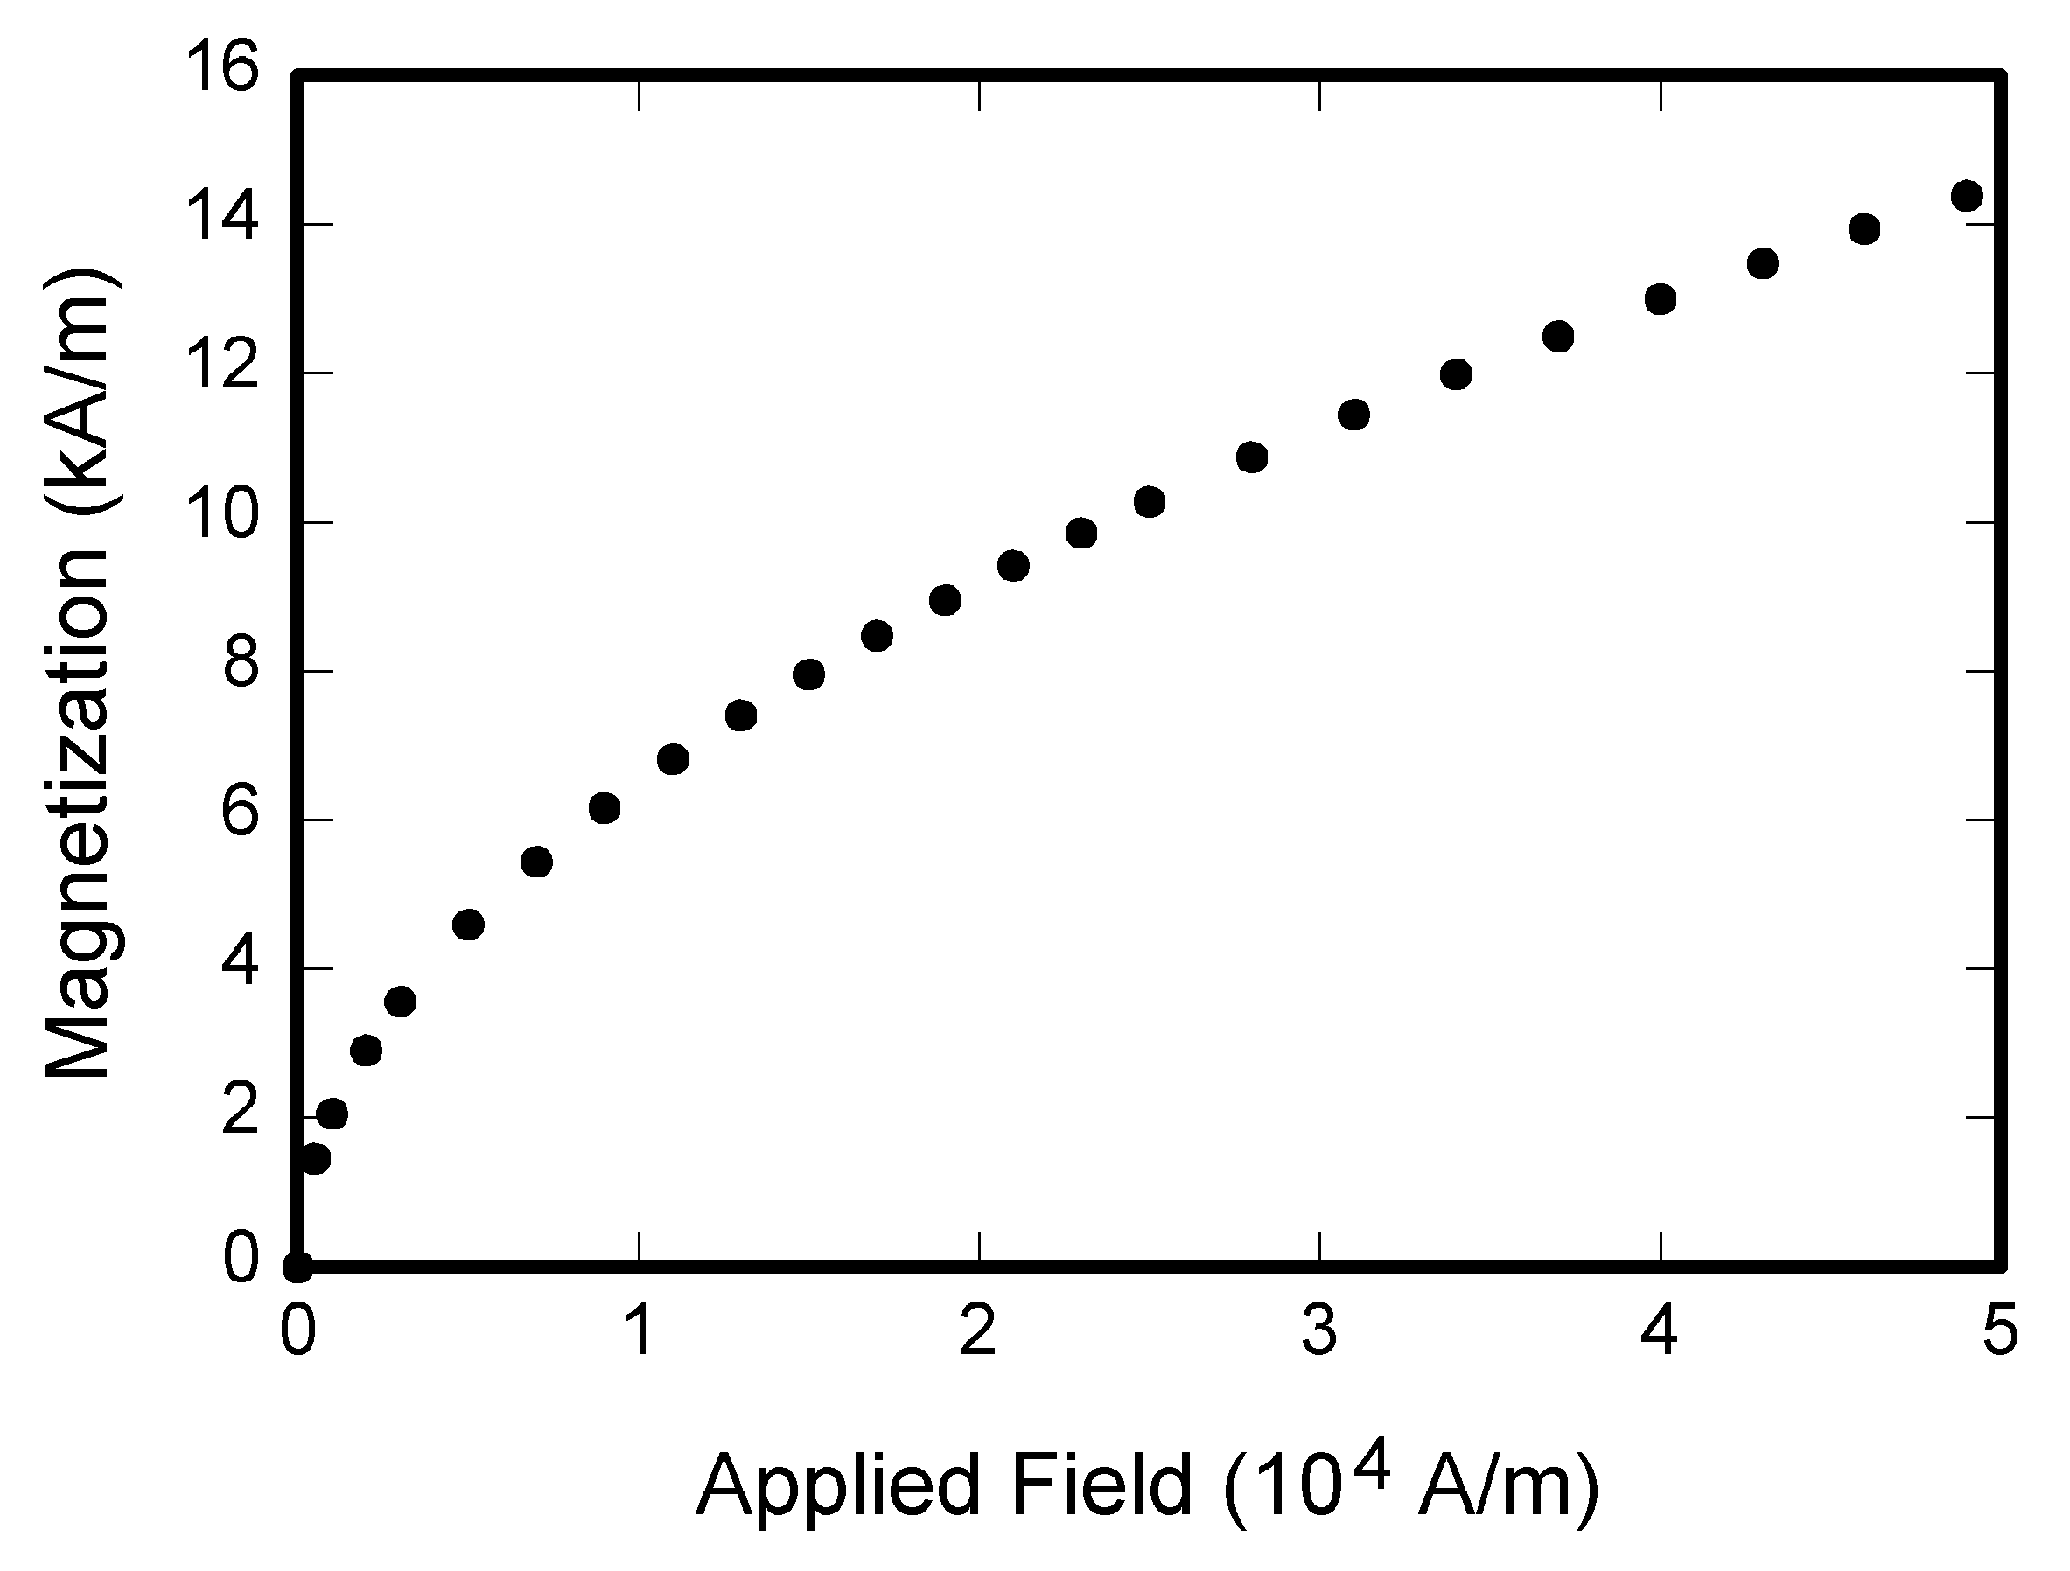
\includegraphics{pics/fig1.png}}
\caption{Example of a figure caption.}
\label{fig}
\end{figure}

Figure Labels: Use 8 point Times New Roman for Figure labels. Use words 
rather than symbols or abbreviations when writing Figure axis labels to 
avoid confusing the reader. As an example, write the quantity 
``Magnetization'', or ``Magnetization, M'', not just ``M''. If including 
units in the label, present them within parentheses. Do not label axes only 
with units. In the example, write ``Magnetization (A/m)'' or ``Magnetization 
\{A[m(1)]\}'', not just ``A/m''. Do not label axes with a ratio of 
quantities and units. For example, write ``Temperature (K)'', not 
``Temperature/K''.

\section*{Acknowledgment}

The preferred spelling of the word ``acknowledgment'' in America is without 
an ``e'' after the ``g''. Avoid the stilted expression ``one of us (R. B. 
G.) thanks $\ldots$''. Instead, try ``R. B. G. thanks$\ldots$''. Put sponsor 
acknowledgments in the unnumbered footnote on the first page.

\section*{References}

Please number citations consecutively within brackets \cite{b1}. The 
sentence punctuation follows the bracket \cite{b2}. Refer simply to the reference 
number, as in \cite{b3}---do not use ``Ref. \cite{b3}'' or ``reference \cite{b3}'' except at 
the beginning of a sentence: ``Reference \cite{b3} was the first $\ldots$''

Number footnotes separately in superscripts. Place the actual footnote at 
the bottom of the column in which it was cited. Do not put footnotes in the 
abstract or reference list. Use letters for table footnotes.

Unless there are six authors or more give all authors' names; do not use 
``et al.''. Papers that have not been published, even if they have been 
submitted for publication, should be cited as ``unpublished'' \cite{b4}. Papers 
that have been accepted for publication should be cited as ``in press'' \cite{b5}. 
Capitalize only the first word in a paper title, except for proper nouns and 
element symbols.

For papers published in translation journals, please give the English 
citation first, followed by the original foreign-language citation \cite{b6}.

\bibliographystyle{IEEEtran}
\bibliography{bibliography}

\vspace{12pt}
\color{red}
IEEE conference templates contain guidance text for composing and formatting conference papers. Please ensure that all template text is removed from your conference paper prior to submission to the conference. Failure to remove the template text from your paper may result in your paper not being published.

\end{document}
